% Options for packages loaded elsewhere
\PassOptionsToPackage{unicode}{hyperref}
\PassOptionsToPackage{hyphens}{url}
\PassOptionsToPackage{dvipsnames,svgnames,x11names}{xcolor}
%
\documentclass[
  letterpaper,
  DIV=11,
  numbers=noendperiod]{scrartcl}

\usepackage{amsmath,amssymb}
\usepackage{lmodern}
\usepackage{iftex}
\ifPDFTeX
  \usepackage[T1]{fontenc}
  \usepackage[utf8]{inputenc}
  \usepackage{textcomp} % provide euro and other symbols
\else % if luatex or xetex
  \usepackage{unicode-math}
  \defaultfontfeatures{Scale=MatchLowercase}
  \defaultfontfeatures[\rmfamily]{Ligatures=TeX,Scale=1}
\fi
% Use upquote if available, for straight quotes in verbatim environments
\IfFileExists{upquote.sty}{\usepackage{upquote}}{}
\IfFileExists{microtype.sty}{% use microtype if available
  \usepackage[]{microtype}
  \UseMicrotypeSet[protrusion]{basicmath} % disable protrusion for tt fonts
}{}
\makeatletter
\@ifundefined{KOMAClassName}{% if non-KOMA class
  \IfFileExists{parskip.sty}{%
    \usepackage{parskip}
  }{% else
    \setlength{\parindent}{0pt}
    \setlength{\parskip}{6pt plus 2pt minus 1pt}}
}{% if KOMA class
  \KOMAoptions{parskip=half}}
\makeatother
\usepackage{xcolor}
\setlength{\emergencystretch}{3em} % prevent overfull lines
\setcounter{secnumdepth}{-\maxdimen} % remove section numbering
% Make \paragraph and \subparagraph free-standing
\ifx\paragraph\undefined\else
  \let\oldparagraph\paragraph
  \renewcommand{\paragraph}[1]{\oldparagraph{#1}\mbox{}}
\fi
\ifx\subparagraph\undefined\else
  \let\oldsubparagraph\subparagraph
  \renewcommand{\subparagraph}[1]{\oldsubparagraph{#1}\mbox{}}
\fi

\usepackage{color}
\usepackage{fancyvrb}
\newcommand{\VerbBar}{|}
\newcommand{\VERB}{\Verb[commandchars=\\\{\}]}
\DefineVerbatimEnvironment{Highlighting}{Verbatim}{commandchars=\\\{\}}
% Add ',fontsize=\small' for more characters per line
\newenvironment{Shaded}{}{}
\newcommand{\AlertTok}[1]{\textcolor[rgb]{0.16,0.16,0.16}{\textbf{\colorbox[rgb]{0.80,0.14,0.11}{#1}}}}
\newcommand{\AnnotationTok}[1]{\textcolor[rgb]{0.60,0.59,0.10}{#1}}
\newcommand{\AttributeTok}[1]{\textcolor[rgb]{0.84,0.60,0.13}{#1}}
\newcommand{\BaseNTok}[1]{\textcolor[rgb]{0.96,0.45,0.00}{#1}}
\newcommand{\BuiltInTok}[1]{\textcolor[rgb]{0.84,0.36,0.05}{#1}}
\newcommand{\CharTok}[1]{\textcolor[rgb]{0.69,0.38,0.53}{#1}}
\newcommand{\CommentTok}[1]{\textcolor[rgb]{0.57,0.51,0.45}{#1}}
\newcommand{\CommentVarTok}[1]{\textcolor[rgb]{0.57,0.51,0.45}{#1}}
\newcommand{\ConstantTok}[1]{\textcolor[rgb]{0.69,0.38,0.53}{\textbf{#1}}}
\newcommand{\ControlFlowTok}[1]{\textcolor[rgb]{0.80,0.14,0.11}{\textbf{#1}}}
\newcommand{\DataTypeTok}[1]{\textcolor[rgb]{0.84,0.60,0.13}{#1}}
\newcommand{\DecValTok}[1]{\textcolor[rgb]{0.96,0.45,0.00}{#1}}
\newcommand{\DocumentationTok}[1]{\textcolor[rgb]{0.60,0.59,0.10}{#1}}
\newcommand{\ErrorTok}[1]{\textcolor[rgb]{0.80,0.14,0.11}{\underline{#1}}}
\newcommand{\ExtensionTok}[1]{\textcolor[rgb]{0.41,0.62,0.42}{\textbf{#1}}}
\newcommand{\FloatTok}[1]{\textcolor[rgb]{0.96,0.45,0.00}{#1}}
\newcommand{\FunctionTok}[1]{\textcolor[rgb]{0.41,0.62,0.42}{#1}}
\newcommand{\ImportTok}[1]{\textcolor[rgb]{0.41,0.62,0.42}{#1}}
\newcommand{\InformationTok}[1]{\textcolor[rgb]{0.16,0.16,0.16}{\colorbox[rgb]{0.51,0.65,0.60}{#1}}}
\newcommand{\KeywordTok}[1]{\textcolor[rgb]{0.24,0.22,0.21}{\textbf{#1}}}
\newcommand{\NormalTok}[1]{\textcolor[rgb]{0.24,0.22,0.21}{#1}}
\newcommand{\OperatorTok}[1]{\textcolor[rgb]{0.24,0.22,0.21}{#1}}
\newcommand{\OtherTok}[1]{\textcolor[rgb]{0.41,0.62,0.42}{#1}}
\newcommand{\PreprocessorTok}[1]{\textcolor[rgb]{0.84,0.36,0.05}{#1}}
\newcommand{\RegionMarkerTok}[1]{\textcolor[rgb]{0.57,0.51,0.45}{\colorbox[rgb]{0.98,0.96,0.84}{#1}}}
\newcommand{\SpecialCharTok}[1]{\textcolor[rgb]{0.69,0.38,0.53}{#1}}
\newcommand{\SpecialStringTok}[1]{\textcolor[rgb]{0.60,0.59,0.10}{#1}}
\newcommand{\StringTok}[1]{\textcolor[rgb]{0.60,0.59,0.10}{#1}}
\newcommand{\VariableTok}[1]{\textcolor[rgb]{0.27,0.52,0.53}{#1}}
\newcommand{\VerbatimStringTok}[1]{\textcolor[rgb]{0.60,0.59,0.10}{#1}}
\newcommand{\WarningTok}[1]{\textcolor[rgb]{0.16,0.16,0.16}{\colorbox[rgb]{0.98,0.74,0.18}{#1}}}

\providecommand{\tightlist}{%
  \setlength{\itemsep}{0pt}\setlength{\parskip}{0pt}}\usepackage{longtable,booktabs,array}
\usepackage{calc} % for calculating minipage widths
% Correct order of tables after \paragraph or \subparagraph
\usepackage{etoolbox}
\makeatletter
\patchcmd\longtable{\par}{\if@noskipsec\mbox{}\fi\par}{}{}
\makeatother
% Allow footnotes in longtable head/foot
\IfFileExists{footnotehyper.sty}{\usepackage{footnotehyper}}{\usepackage{footnote}}
\makesavenoteenv{longtable}
\usepackage{graphicx}
\makeatletter
\def\maxwidth{\ifdim\Gin@nat@width>\linewidth\linewidth\else\Gin@nat@width\fi}
\def\maxheight{\ifdim\Gin@nat@height>\textheight\textheight\else\Gin@nat@height\fi}
\makeatother
% Scale images if necessary, so that they will not overflow the page
% margins by default, and it is still possible to overwrite the defaults
% using explicit options in \includegraphics[width, height, ...]{}
\setkeys{Gin}{width=\maxwidth,height=\maxheight,keepaspectratio}
% Set default figure placement to htbp
\makeatletter
\def\fps@figure{htbp}
\makeatother

% Load packages
\usepackage{geometry} % For setting page dimensions
\usepackage{xcolor} % For defining and using colors
\usepackage{eso-pic} % For adding elements to each page
\usepackage{fancyhdr} % For custom page headers and footers
\usepackage{sectsty} % For styling section and chapter titles
\usepackage{fontspec} % For custom font handling
\usepackage{titlesec} % For customizing section titles
\usepackage{listings} % For including code listings
\usepackage{setspace} % For adjusting line spacing
\usepackage{mfirstuc}

% Define colors
\definecolor{light}{HTML}{D73F09}
\definecolor{highlight}{HTML}{800080}
\definecolor{dark}{HTML}{330033}

%% Define and import custom fonts
\setsansfont{Stratum2}[
    Path=_extensions/OSULatexTheme/Stratum2/,
    Scale=1,
    Extension = .ttf,
    UprightFont=* Medium,
    BoldFont=* Bold,
    ItalicFont=* Regular,
    ]

\setmainfont{Kievit}[
    Path=_extensions/OSULatexTheme/Kievit/,
    Scale=1,
    Extension = .ttf,
    UprightFont=* Regular,
    BoldFont=* Bold,
    ItalicFont=* Black Italic,
    ]

% Define page setup variables
\newcommand{\mypapersize}{a4paper}
\newcommand{\mytotal}{170mm,257mm}
\newcommand{\myleft}{20mm}
\newcommand{\mytop}{15mm}
\newcommand{\mybottom}{15mm}
\newcommand{\myright}{30mm}

% Set page setup
\geometry{\mypapersize, total={\mytotal}, left=\myleft, top=\mytop, bottom=\mybottom, right=\myright}

% Title alignment
\makeatletter
\renewcommand{\maketitle}{\bgroup\setlength{\parindent}{0pt}
\begin{flushleft}
  {\sffamily\fontsize{28}{5}\textbf{\capitalisewords{\@title}}} \vspace{0.3cm} \newline
  {\large\@author} \newline
  {\large\today} \newline % Include the full date here
  {\large {\@subtitle}} \vspace{-0.3cm}
\end{flushleft}\egroup
}

% Set line spacing
\newcommand{\mylinespacing}{1.25} % Adjust the value as needed
\setstretch{\mylinespacing}

% Section styles
% Section font settings
\titleformat{\section}{\sffamily\fontsize{23}{20}\bfseries}{\thesection}{1em}{}[{\titlerule[2.5pt]}]
\titleformat{\subsection}{\sffamily\fontsize{19}{15}\bfseries}{\thesubsection}{1em}{}[{\titlerule[1pt]}]
\titleformat{\subsubsection}{\sffamily\fontsize{15}{10}\bfseries}{\thesubsubsection}{1em}{}[{\titlerule[0.5pt]}]

% Logo and bar placement
\AddToShipoutPicture{% 
    \AtPageLowerLeft{% 
        \put(\LenToUnit{\dimexpr\paperwidth-2.6cm},26.7cm){% 
            \color{light}\rule{3cm}{3cm}% Adjust the height as needed
        }%
    }%
    \AtPageLowerLeft{% start the bar at the bottom right of the page
        \put(\LenToUnit{\dimexpr\paperwidth-2.45cm},27cm){% move it to the top right
            \color{light}
\includegraphics[width=2.35cm]{_extensions/OSULatexTheme/logo2.png}
        }%
    }%
}

% Other Page Styling
\fancypagestyle{mystyle}{
  \fancyhf{}
  \renewcommand\headrulewidth{2.5pt}
  \fancyfoot[R]{\fontsize{20}{12}\selectfont\thepage} 
  \fancyfootoffset{2.5cm}
  \setlength{\footskip}{20pt}
}

\pagestyle{mystyle}
\KOMAoption{captions}{tableheading}
\makeatletter
\makeatother
\makeatletter
\makeatother
\makeatletter
\@ifpackageloaded{caption}{}{\usepackage{caption}}
\AtBeginDocument{%
\ifdefined\contentsname
  \renewcommand*\contentsname{Table of contents}
\else
  \newcommand\contentsname{Table of contents}
\fi
\ifdefined\listfigurename
  \renewcommand*\listfigurename{List of Figures}
\else
  \newcommand\listfigurename{List of Figures}
\fi
\ifdefined\listtablename
  \renewcommand*\listtablename{List of Tables}
\else
  \newcommand\listtablename{List of Tables}
\fi
\ifdefined\figurename
  \renewcommand*\figurename{Figure}
\else
  \newcommand\figurename{Figure}
\fi
\ifdefined\tablename
  \renewcommand*\tablename{Table}
\else
  \newcommand\tablename{Table}
\fi
}
\@ifpackageloaded{float}{}{\usepackage{float}}
\floatstyle{ruled}
\@ifundefined{c@chapter}{\newfloat{codelisting}{h}{lop}}{\newfloat{codelisting}{h}{lop}[chapter]}
\floatname{codelisting}{Listing}
\newcommand*\listoflistings{\listof{codelisting}{List of Listings}}
\makeatother
\makeatletter
\@ifpackageloaded{caption}{}{\usepackage{caption}}
\@ifpackageloaded{subcaption}{}{\usepackage{subcaption}}
\makeatother
\makeatletter
\@ifpackageloaded{tcolorbox}{}{\usepackage[many]{tcolorbox}}
\makeatother
\makeatletter
\@ifundefined{shadecolor}{\definecolor{shadecolor}{HTML}{000000}}
\makeatother
\makeatletter
\makeatother
\ifLuaTeX
  \usepackage{selnolig}  % disable illegal ligatures
\fi
\IfFileExists{bookmark.sty}{\usepackage{bookmark}}{\usepackage{hyperref}}
\IfFileExists{xurl.sty}{\usepackage{xurl}}{} % add URL line breaks if available
\urlstyle{same} % disable monospaced font for URLs
\hypersetup{
  pdftitle={Homework 2},
  pdfauthor={Brian Cervantes Alvarez},
  colorlinks=true,
  linkcolor={highlight},
  filecolor={Maroon},
  citecolor={Blue},
  urlcolor={highlight},
  pdfcreator={LaTeX via pandoc}}

\title{Homework 2}
\usepackage{etoolbox}
\makeatletter
\providecommand{\subtitle}[1]{% add subtitle to \maketitle
  \apptocmd{\@title}{\par {\large #1 \par}}{}{}
}
\makeatother
\subtitle{ST552: Statistical Methods}
\author{Brian Cervantes Alvarez}
\date{1/26/23}

\begin{document}
\maketitle
\ifdefined\Shaded\renewenvironment{Shaded}{\begin{tcolorbox}[enhanced, boxrule=0pt, breakable, borderline west={3pt}{0pt}{shadecolor}, interior hidden, frame hidden, sharp corners]}{\end{tcolorbox}}\fi

\hypertarget{question-1}{%
\section{Question 1}\label{question-1}}

\hypertarget{part-a}{%
\subsection{Part A}\label{part-a}}

Here is the simple linear model:

\[y_i = \beta_0 + \beta_{1}x_i + \epsilon_i\]

The linear regression model in matrix form represented as:

\[ Y = X\beta + \epsilon \]

where:

\begin{itemize}
\tightlist
\item
  \(Y\) is the vector of responses \(y_i\) for \(i = 1\) to \(n\).
\item
  \(X\) is the matrix of predictors with each row corresponding to an
  observation and each column to a predictor.
\item
  \(\beta\) is the vector of coefficients
  \(\beta_0, \beta_1, ..., \beta_p\) where \(p\) is the number of
  predictors; in our case, \(p = 1, \{\beta_0, \beta_1\}\).
\item
  \(\epsilon\) is the vector of random errors.
\end{itemize}

\[ Y = \begin{bmatrix} y_1 \\ y_2 \\ \vdots \\ y_n \end{bmatrix}, \quad X = \begin{bmatrix} 1 & x_1 \\ 1 & x_2 \\ \vdots & \vdots \\ 1 & x_n \end{bmatrix}, \quad \beta = \begin{bmatrix} \beta_0 \\ \beta_1 \end{bmatrix}, \quad \epsilon = \begin{bmatrix} \epsilon_1 \\ \epsilon_2 \\ \vdots \\ \epsilon_n \end{bmatrix} \]

Therefore, the matrices and vectors become:

\[ Y = X\beta + \epsilon, \quad \begin{bmatrix} y_1 \\ y_2 \\ \vdots \\ y_n \end{bmatrix} = \begin{bmatrix} 1 & x_1 \\ 1 & x_2 \\ \vdots & \vdots \\ 1 & x_n \end{bmatrix} \begin{bmatrix} \beta_0 \\ \beta_1 \end{bmatrix} + \begin{bmatrix} \epsilon_1 \\ \epsilon_2 \\ \vdots \\ \epsilon_n \end{bmatrix} \]

\newpage{}

\hypertarget{part-b}{%
\subsection{Part B}\label{part-b}}

\hypertarget{solution-for-xtx}{%
\subsubsection{\texorpdfstring{Solution for
\(X^TX\)}{Solution for X\^{}TX}}\label{solution-for-xtx}}

We know \(X\), and \(X^T\) can be easily transformed as the following:

\[ X = \begin{bmatrix} 1 & x_1 \\ 1 & x_2 \\ \vdots & \vdots \\ 1 & x_n \end{bmatrix}, \quad  X^T = \begin{bmatrix} 1 & 1 & \dots & 1 \\ x_1 & x_2 & \dots & x_n \end{bmatrix} \]

Now, we multiply \(X^T\) by \(X\). Then, by using matrix multiplication,
it becomes a \(2x2\) square matrix, we get our solution:

\[X^TX = \begin{bmatrix} 1 & 1 & \dots & 1 \\ x_1 & x_2 & \dots & x_n \end{bmatrix} \begin{bmatrix} 1 & x_1 \\ 1 & x_2 \\ \vdots & \vdots \\ 1 & x_n \end{bmatrix} = \begin{bmatrix} n & \sum_{i=1}^{n}x_i \\ \sum_{i=1}^{n}x_i & \sum_{i=1}^{n}x_i^2 \end{bmatrix} = \begin{bmatrix} n & n\bar{x} \\ n\bar{x} & \sum_{i=1}^{n}x_i^2 \end{bmatrix}\]

\hypertarget{solution-for-xty}{%
\subsubsection{\texorpdfstring{Solution for
\(X^TY\)}{Solution for X\^{}TY}}\label{solution-for-xty}}

Given \(X\) and \(Y\), we can solve for \(X^TY\) as follows::

\[ X = \begin{bmatrix} 1 & x_1 \\ 1 & x_2 \\ \vdots & \vdots \\ 1 & x_n \end{bmatrix}, \quad Y = \begin{bmatrix} y_1 \\ y_2 \\ \vdots \\ y_n \end{bmatrix} \Rightarrow  X^TY = \begin{bmatrix} 1 & 1 & \dots & 1 \\ x_1 & x_2 & \dots & x_n \end{bmatrix} \begin{bmatrix} y_1 \\ y_2 \\ \vdots \\ y_n \end{bmatrix} = \begin{bmatrix} \sum_{i=1}^{n}y_i \\ \sum_{i=1}^{n}x_iy_i \end{bmatrix} = \begin{bmatrix} n\bar{y} \\ \sum_{i=1}^{n}x_iy_i \end{bmatrix}\]

\hypertarget{solution-for-xtx-1}{%
\subsubsection{\texorpdfstring{Solution for
\((X^TX)^{-1}\)}{Solution for (X\^{}TX)\^{}\{-1\}}}\label{solution-for-xtx-1}}

Recall that the inverse of a 2x2 matrix
\(\begin{bmatrix} a & b \\ c & d \end{bmatrix}\) is given by:

\[ \begin{bmatrix} a & b \\ c & d \end{bmatrix}^{-1} = \frac{1}{ad - bc} \begin{bmatrix} d & -b \\ -c & a \end{bmatrix} \]

Given we know \(X^TX\), we can use that to solve for \((X^TX)^{-1}\):
\[ (X^TX)^{-1} = \begin{bmatrix} n & n\bar{x} \\ n\bar{x} & \sum_{i=1}^{n}x_i^2 \end{bmatrix}^{-1} = \frac{1}{nS_{xx}} \begin{bmatrix} \sum_{i=1}^{n}x_i^2 & -n\bar{x} \\ -n\bar{x} & n \end{bmatrix} = \frac{1}{S_{xx}} \begin{bmatrix} \frac{1}{n}\sum_{i=1}^{n}x_i^2 & -\bar{x} \\ -\bar{x} & 1 \end{bmatrix}\]

\newpage{}

\hypertarget{part-c}{%
\subsection{Part C}\label{part-c}}

Least squares estimates \(\hat{\beta}\) would be computed like this:

\[
\begin{align*}
\hat{\beta} &= (X^TX)^{-1}X^TY \\
&= \frac{1}{S_{xx}} \begin{bmatrix} \frac{1}{n}\sum_{i=1}^{n}x_i^2 & -\bar{x} \\ -\bar{x} & 1 \end{bmatrix} \begin{bmatrix} n\bar{y} \\ \sum_{i=1}^{n}x_iy_i \end{bmatrix} \\
&= \frac{1}{S_{xx}} \begin{bmatrix} \bar{y}\sum_{i=1}^nx_{i}^2 -\bar{x}\sum_{i=1}^nx_{i}y_i \\ \sum_{i=1}^nx_{i}y_i -n\bar{x}\bar{y} \end{bmatrix} 
\end{align*}
\]

\newpage{}

\hypertarget{part-d}{%
\subsection{Part D}\label{part-d}}

\newpage{}

\hypertarget{problem-2}{%
\section{Problem 2}\label{problem-2}}

\hypertarget{part-a-1}{%
\subsection{Part A}\label{part-a-1}}

\begin{Shaded}
\begin{Highlighting}[]
\FunctionTok{library}\NormalTok{(faraway)}
\FunctionTok{library}\NormalTok{(ggplot2)}
\FunctionTok{data}\NormalTok{(teengamb)}
\NormalTok{ds }\OtherTok{\textless{}{-}}\NormalTok{ teengamb}

\CommentTok{\# Construct matrix X and response vector Y}
\NormalTok{X }\OtherTok{\textless{}{-}} \FunctionTok{cbind}\NormalTok{(}\DecValTok{1}\NormalTok{, ds}\SpecialCharTok{$}\NormalTok{sex, ds}\SpecialCharTok{$}\NormalTok{status, ds}\SpecialCharTok{$}\NormalTok{income, ds}\SpecialCharTok{$}\NormalTok{verbal)}
\NormalTok{Y }\OtherTok{\textless{}{-}}\NormalTok{ teengamb}\SpecialCharTok{$}\NormalTok{gamble}
\end{Highlighting}
\end{Shaded}

\newpage{}

\hypertarget{part-b-1}{%
\subsection{Part B}\label{part-b-1}}

\begin{Shaded}
\begin{Highlighting}[]
\CommentTok{\# Find the least squares estimates of the regression coefficients}
\NormalTok{betaHat }\OtherTok{\textless{}{-}} \FunctionTok{solve}\NormalTok{(}\FunctionTok{t}\NormalTok{(X) }\SpecialCharTok{\%*\%}\NormalTok{ X) }\SpecialCharTok{\%*\%} \FunctionTok{t}\NormalTok{(X) }\SpecialCharTok{\%*\%}\NormalTok{ Y}
\end{Highlighting}
\end{Shaded}

\newpage{}

\hypertarget{part-c-1}{%
\subsection{Part C}\label{part-c-1}}

\begin{Shaded}
\begin{Highlighting}[]
\CommentTok{\# Find the fitted values and residuals}
\NormalTok{fittedVals }\OtherTok{\textless{}{-}}\NormalTok{ X }\SpecialCharTok{\%*\%}\NormalTok{ betaHat}
\NormalTok{residuals }\OtherTok{\textless{}{-}}\NormalTok{ Y }\SpecialCharTok{{-}}\NormalTok{ fittedVals}

\CommentTok{\# Plot residuals against fitted values}
\FunctionTok{plot}\NormalTok{(fittedVals, residuals, }\AttributeTok{main =} \StringTok{"Residuals vs Fitted Values"}\NormalTok{, }
     \AttributeTok{xlab =} \StringTok{"Fitted Values"}\NormalTok{, }\AttributeTok{ylab =} \StringTok{"Residuals"}\NormalTok{)}
\end{Highlighting}
\end{Shaded}

\begin{figure}[H]

{\centering 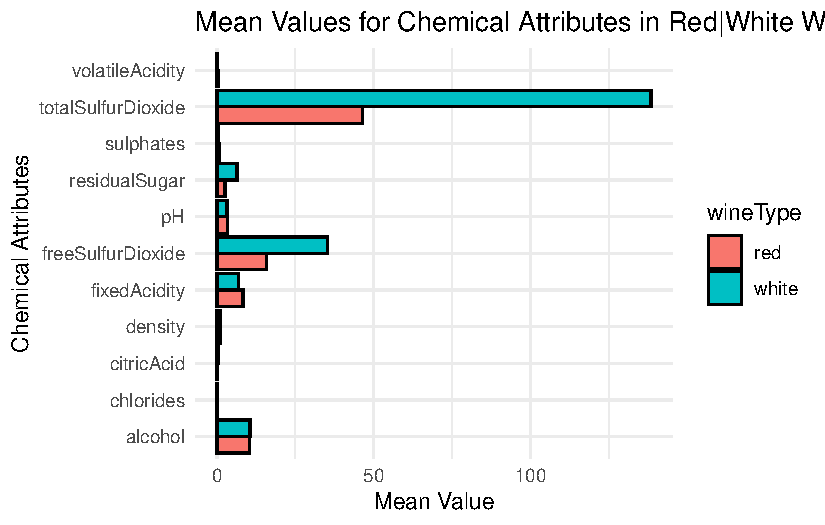
\includegraphics{ST552-HW2-BCA_files/figure-pdf/unnamed-chunk-3-1.pdf}

}

\end{figure}

\newpage{}

\hypertarget{part-d-1}{%
\subsection{Part D}\label{part-d-1}}

\begin{Shaded}
\begin{Highlighting}[]
\CommentTok{\# Fit the model}
\NormalTok{model }\OtherTok{\textless{}{-}} \FunctionTok{lm}\NormalTok{(}\AttributeTok{data =}\NormalTok{ ds, gamble }\SpecialCharTok{\textasciitilde{}}\NormalTok{ sex }\SpecialCharTok{+}\NormalTok{ status }\SpecialCharTok{+}\NormalTok{ income }\SpecialCharTok{+}\NormalTok{ verbal)}
\FunctionTok{summary}\NormalTok{(model)}
\end{Highlighting}
\end{Shaded}

\begin{verbatim}

Call:
lm(formula = gamble ~ sex + status + income + verbal, data = ds)

Residuals:
    Min      1Q  Median      3Q     Max 
-51.082 -11.320  -1.451   9.452  94.252 

Coefficients:
             Estimate Std. Error t value Pr(>|t|)    
(Intercept)  22.55565   17.19680   1.312   0.1968    
sex         -22.11833    8.21111  -2.694   0.0101 *  
status        0.05223    0.28111   0.186   0.8535    
income        4.96198    1.02539   4.839 1.79e-05 ***
verbal       -2.95949    2.17215  -1.362   0.1803    
---
Signif. codes:  0 '***' 0.001 '**' 0.01 '*' 0.05 '.' 0.1 ' ' 1

Residual standard error: 22.69 on 42 degrees of freedom
Multiple R-squared:  0.5267,    Adjusted R-squared:  0.4816 
F-statistic: 11.69 on 4 and 42 DF,  p-value: 1.815e-06
\end{verbatim}

\hypertarget{part-e}{%
\subsection{Part E}\label{part-e}}

MY INTERPRETATION IS

\newpage{}

\hypertarget{problem-3}{%
\section{Problem 3}\label{problem-3}}

\hypertarget{part-a-2}{%
\subsection{Part A}\label{part-a-2}}

Here is the model that we are going to use:

\[\text{Weekly Wages} = \beta_0 + \beta_1 \times \text{Education} + \beta_2 \times \text{Experience}\]

\newpage{}

\hypertarget{part-b-2}{%
\subsection{Part B}\label{part-b-2}}

\begin{Shaded}
\begin{Highlighting}[]
\FunctionTok{data}\NormalTok{(uswages)}
\NormalTok{ds }\OtherTok{\textless{}{-}}\NormalTok{ uswages}

\CommentTok{\# Fit the model}
\NormalTok{expEducationModel }\OtherTok{\textless{}{-}} \FunctionTok{lm}\NormalTok{(}\AttributeTok{data =}\NormalTok{ ds, wage }\SpecialCharTok{\textasciitilde{}}\NormalTok{ educ }\SpecialCharTok{+}\NormalTok{ exper)}
\FunctionTok{summary}\NormalTok{(expEducationModel)}
\end{Highlighting}
\end{Shaded}

\begin{verbatim}

Call:
lm(formula = wage ~ educ + exper, data = ds)

Residuals:
    Min      1Q  Median      3Q     Max 
-1018.2  -237.9   -50.9   149.9  7228.6 

Coefficients:
             Estimate Std. Error t value Pr(>|t|)    
(Intercept) -242.7994    50.6816  -4.791 1.78e-06 ***
educ          51.1753     3.3419  15.313  < 2e-16 ***
exper          9.7748     0.7506  13.023  < 2e-16 ***
---
Signif. codes:  0 '***' 0.001 '**' 0.01 '*' 0.05 '.' 0.1 ' ' 1

Residual standard error: 427.9 on 1997 degrees of freedom
Multiple R-squared:  0.1351,    Adjusted R-squared:  0.1343 
F-statistic:   156 on 2 and 1997 DF,  p-value: < 2.2e-16
\end{verbatim}

\newpage{}

\hypertarget{part-c-2}{%
\subsection{Part C}\label{part-c-2}}

\begin{Shaded}
\begin{Highlighting}[]
\CommentTok{\# Fit the linear model}
\NormalTok{expSmsaModel }\OtherTok{\textless{}{-}} \FunctionTok{lm}\NormalTok{(wage }\SpecialCharTok{\textasciitilde{}}\NormalTok{ exper }\SpecialCharTok{+}\NormalTok{ smsa, }\AttributeTok{data =}\NormalTok{ ds)}
\CommentTok{\# Extract model coefficients}
\NormalTok{int }\OtherTok{\textless{}{-}} \FunctionTok{coef}\NormalTok{(expSmsaModel)[}\DecValTok{1}\NormalTok{]}
\NormalTok{coefSmsa0 }\OtherTok{\textless{}{-}} \FunctionTok{coef}\NormalTok{(expSmsaModel)[}\DecValTok{2}\NormalTok{]}
\NormalTok{coefSmsa1 }\OtherTok{\textless{}{-}} \FunctionTok{coef}\NormalTok{(expSmsaModel)[}\DecValTok{2}\NormalTok{] }\SpecialCharTok{+} \FunctionTok{coef}\NormalTok{(expSmsaModel)[}\DecValTok{3}\NormalTok{]}
\CommentTok{\# For regression lines}
\NormalTok{regressionDs }\OtherTok{\textless{}{-}} \FunctionTok{data.frame}\NormalTok{(}\AttributeTok{exper =} \FunctionTok{seq}\NormalTok{(}\FunctionTok{min}\NormalTok{(ds}\SpecialCharTok{$}\NormalTok{exper),}\FunctionTok{max}\NormalTok{(ds}\SpecialCharTok{$}\NormalTok{exper), }
                                       \AttributeTok{length.out =} \DecValTok{100}\NormalTok{))}
\NormalTok{regressionDs}\SpecialCharTok{$}\NormalTok{wageSmsa0 }\OtherTok{\textless{}{-}}\NormalTok{ int }\SpecialCharTok{+}\NormalTok{ coefSmsa0 }\SpecialCharTok{*}\NormalTok{ regressionDs}\SpecialCharTok{$}\NormalTok{exper}
\NormalTok{regressionDs}\SpecialCharTok{$}\NormalTok{wageSmsa1 }\OtherTok{\textless{}{-}}\NormalTok{ int }\SpecialCharTok{+}\NormalTok{ coefSmsa1 }\SpecialCharTok{*}\NormalTok{ regressionDs}\SpecialCharTok{$}\NormalTok{exper}
\CommentTok{\# Plot}
\FunctionTok{ggplot}\NormalTok{(}\AttributeTok{data =}\NormalTok{ ds, }\FunctionTok{aes}\NormalTok{(}\AttributeTok{x =}\NormalTok{ exper, }\AttributeTok{y =}\NormalTok{ wage, }\AttributeTok{color =} \FunctionTok{factor}\NormalTok{(smsa))) }\SpecialCharTok{+}
  \FunctionTok{geom\_point}\NormalTok{(}\AttributeTok{alpha =} \FloatTok{0.3}\NormalTok{, }\AttributeTok{size =} \DecValTok{2}\NormalTok{) }\SpecialCharTok{+}
  \FunctionTok{geom\_line}\NormalTok{(}\AttributeTok{data =}\NormalTok{ regressionDs, }\FunctionTok{aes}\NormalTok{(}\AttributeTok{x =}\NormalTok{ exper, }\AttributeTok{y =}\NormalTok{ wageSmsa0), }
            \AttributeTok{color =} \StringTok{"chocolate4"}\NormalTok{) }\SpecialCharTok{+}
  \FunctionTok{geom\_line}\NormalTok{(}\AttributeTok{data =}\NormalTok{ regressionDs, }\FunctionTok{aes}\NormalTok{(}\AttributeTok{x =}\NormalTok{ exper, }\AttributeTok{y =}\NormalTok{ wageSmsa1), }
            \AttributeTok{color =} \StringTok{"cyan3"}\NormalTok{) }\SpecialCharTok{+}
  \FunctionTok{labs}\NormalTok{(}\AttributeTok{x =} \StringTok{"Years of Experience"}\NormalTok{, }\AttributeTok{y =} \StringTok{"Weekly Wages"}\NormalTok{, }\AttributeTok{color =} \StringTok{"SMSA"}\NormalTok{) }\SpecialCharTok{+}
  \FunctionTok{scale\_color\_manual}\NormalTok{(}\AttributeTok{values =} \FunctionTok{c}\NormalTok{(}\StringTok{"0"} \OtherTok{=} \StringTok{"chocolate4"}\NormalTok{, }
                                \StringTok{"1"} \OtherTok{=} \StringTok{"cyan3"}\NormalTok{)) }\SpecialCharTok{+}
  \FunctionTok{theme\_minimal}\NormalTok{()}
\end{Highlighting}
\end{Shaded}

\begin{figure}[H]

{\centering 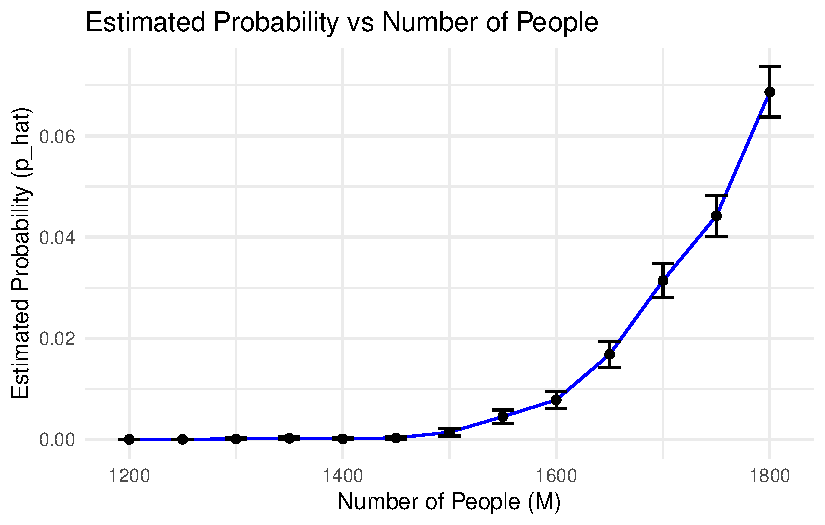
\includegraphics{ST552-HW2-BCA_files/figure-pdf/unnamed-chunk-6-1.pdf}

}

\end{figure}



\end{document}
